\documentclass[12pt, answers]{exam}
\usepackage{tikz}
\usepackage{hyperref}
\usepackage[a4paper, total={6in, 9in}]{geometry}
\usepackage{caption}
\usepackage{algpseudocodex}
\usepackage{algorithm}
\usepackage{amsmath}
\usepackage{amsfonts}
\usepackage{amssymb}
\usepackage{mathtools}
\usepackage{mathrsfs}
\usepackage{listings}
\usepackage{graphicx}
\usepackage{setspace}
\usepackage{subfiles}
\usepackage{xcolor}
\usepackage{multirow}
\usepackage{xepersian}
\settextfont[Scale = 1.0 ,
Path = ../fonts/ ,
BoldFont = *Bd ,
ItalicFont = *It ,
BoldItalicFont = *BdIt ,
Extension = .ttf
]{XB Yas}


\definecolor{codegreen}{rgb}{0,0.6,0}
\definecolor{codegray}{rgb}{0.5,0.5,0.5}
\definecolor{codepurple}{rgb}{0.58,0,0.82}
\definecolor{backcolour}{rgb}{0.95,0.95,0.92}


\lstdefinestyle{mystyle}{
    backgroundcolor=\color{backcolour},   
    commentstyle=\color{codegreen},
    keywordstyle=\color{magenta},
    numberstyle=\tiny\color{codegray},
    stringstyle=\color{codepurple},
    basicstyle=\ttfamily\footnotesize,
    breakatwhitespace=false,         
    breaklines=true,                 
    captionpos=b,                    
    keepspaces=true,                 
    numbers=left,                    
    numbersep=5pt,                  
    showspaces=false,                
    showstringspaces=false,
    showtabs=false,                  
    tabsize=2
}

\lstset{style=mystyle}


\pointpoints{نمره}{نمره}
\renewcommand{\solutiontitle}{\noindent\textbf{پاسخ:}\par}
\newcommand{\class}{اصول سیستم‌های عامل}
\newcommand{\term}{نیم‌سال اول ۰۴-۰۵}
\newcommand{\college}{دانشکده ریاضی و آمار}
\newcommand{\prof}{استاد: دکتر رفیعی}
\newcommand{\group}{\textcolor{red}{نام دانشجو}}

\begin{document}

\pagestyle{head}
\firstpageheader{}{}{}
\runningheader{صفحه \thepage\ از \numpages}{}{\class}
\runningheadrule
\begin{tabular}{p{.7\textwidth} l}
    \multicolumn{2}{c}{\textbf{به نام خدا}}                                            \\
                    & \multirow{2}{*}{
\includegraphics[scale=0.2]{../UILOGO.png}} \\
    \textbf{\class} &                                                                  \\
    \textbf{\term}  &                                                                  \\
    \textbf{\prof}  &                                                                  \\
    \textbf{\group} &                                                                  \\
                    & \textbf{\college}                                                \\
    % & \textbf{\todaydate} \\
    % & \textbf{\deadline} \\ \\
\end{tabular}\\
\rule[1ex]{\textwidth}{.1pt}

\begin{center}
    \textbf{\lr{Problem Set 2}}
\end{center}


\begin{questions}

    %% 1

    \question[5] پاسخ مناسب بدهید.
\begin{parts}
    \part[1] به تعداد فرآیندهای جاری در حافظه‌ی اصلی
    \dots \dots \dots \
    گفته می‌شود

    \part[1] ساختار داده مربوط به صف فرآیندها
    \dots \dots \dots \
    نام دارد.

    \part[1] مولفه Parent PID مربوط به
    systemd
    برابر با
    \dots \dots \dots \
    است.

    \part[2] Mounting فرآیندی است که
    \dots \dots \dots \
    .


\end{parts}

    \begin{solution}
        \textcolor{red}{پاسخ خود را اینجا بنویسید.}
    \end{solution}

    \pagebreak

    %% 2

    \question[30] به صورت کامل پاسخ دهید:
\begin{parts}
	\part[5] با توجه به توضیح قسمت الف، آیا ممکن است که فرآیندی پس از یتیم شدن به زامبی تبدیل شود؟ توضیح دهید.
	\part[5] پنج سناریو بیان کنید که در آن یک فرآیند از حالت خاتمه به حالت مسدود برود.
    \part[10] توضیح دهید که بعد از یتیم شدن یک فرآیند، سیستم‌عامل چه تدبیری می‌اندیشد.
    
    \part[10] با توجه به اینکه فرآیند زامبی منابع تخصیص یافته به خود را رها کرده
    و عملا خاتمه یافته است، آیا ممکن است داشتن تعداد زیادی فرآیند زامبی اختلالی در سیستم ایجاد کند؟ پاسخ خود را شرح دهید.
    

\end{parts}
    \begin{solution}
        \textcolor{red}{پاسخ خود را اینجا بنویسید.}
    \end{solution}

    \pagebreak

  

    %% 4

    \question به سؤالات زیر پاسخ کامل دهید:

\begin{parts}
    \part[10]  فرض کنید تنها امکان پیاده‌سازی فرآیندهای چندنخی در فضای کاربر (و نه فضای کرنل) مهیاست.
    با این فرض، بزرگ‌ترین مزیت و بزرگ‌ترین عیب چنین پیاده‌سازی از نخ‌ها را چه می‌دانید؟ تحلیل کنید.

    \part[10] با توجه به شکل ۱؛ نمونه درخت فرآیند در سیستم‌عامل لینوکس در اسلاید ۱۰:
    \begin{center}
        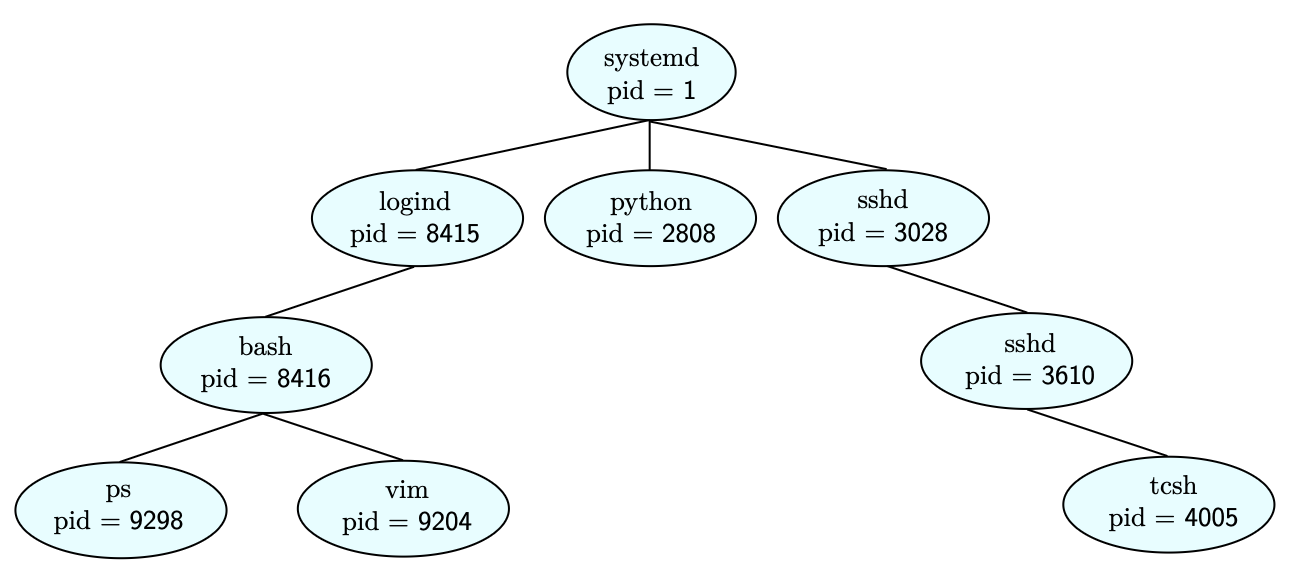
\includegraphics[width=0.8\textwidth]{images/PID_Tree.png}
    \end{center}
    \begin{parts}
        \part در تصویر، چند رابطه‌ی پدر–فرزندی \lr{(Parent–Child Relationship)} وجود دارد؟
        اگر فرآیند {\lr{systemd}} سه فرآیند جدید دیگر ایجاد کند، ساختار درخت چند سطح و چند گره خواهد داشت؟ پاسخ را با تحلیل ساختار فعلی بدهید.

        \part تعداد کل فرآیندها و سطوح درخت را مشخص کنید.
        همچنین بگویید اگر فرآیند {\lr{logind}} خاتمه یابد، دقیقاً چه فرآیندهایی تحت تأثیر قرار می‌گیرند؟
    \end{parts}

    \part[15] در یک سیستم‌عامل فرضی، طراح تصمیم گرفته امکان انتقال یک فرآیند از حالت {\lr{Terminated}} به {\lr{Blocked}} را فراهم کند تا از آن در برخی کاربردهای خاص (مثل بازیابی یا خطایابی) استفاده شود.
    تحلیل کنید که اجرای چنین تصمیمی چه تغییراتی در ساختار سیستم‌عامل و چه چالش‌هایی در زمینه‌ی مدیریت منابع و پایداری فرآیندها به همراه دارد.
    همچنین توضیح دهید در چه شرایطی چنین طراحی می‌تواند موجه یا خطرناک باشد.

\end{parts}

    \begin{solution}
        \textcolor{red}{پاسخ خود را اینجا بنویسید.}
    \end{solution}

    \pagebreak

    %% 5

    \question[20] برنامه زیر را در نظر گرفته و با توجه به ویژگی‌های فراخوان سیستمی ،fork
درخت فرآیند‌های آن را رسم کنید.
\begin{latin}
    \begin{lstlisting}[language=C]
#include <unistd.h>

int main() {
    pid_t p = fork();
    if (p == 0) {
        fork();
    } else {
        pid_t p2 = fork();
        if (p2 == 0) {
            fork();
        }
        fork();
    }
    fork();
    return 0;
}
\end{lstlisting}
\end{latin}

    \begin{solution}
        \textcolor{red}{پاسخ خود را اینجا بنویسید.}
    \end{solution}

    \pagebreak

    %% 6

    \question[30] با توجه به کد زیر،‌ ابتدا مشخص کنید که آیا میتوان در هریک از بخش‌های سوال و با استفاده از فراخوان سیستمی wait
خروجی مد نظر را چاپ کرد و سپس جواب خود را توجیه کنید.

\begin{latin}
    \begin{lstlisting}[language=C]
#include <unistd.h>
#include <stdio.h>

int main() {
    pid_t p = fork();
    if (p == 0) {
        for(int i = 0; i < 100; i++) {
            printf("C");
            printf("D");
        }
    } else {
        for(int i = 0; i < 100; i++) {
            printf("A");
            printf("B");
        }
    }
    return 0;
}
\end{lstlisting}
\end{latin}

\begin{enumerate}
    \item $C^* A^* B^* D$
    \item $(CD)^*(AB)^*$
    \item $A(CD)^*B$
    \item $BCDA$
\end{enumerate}

    \begin{solution}
        \textcolor{red}{پاسخ خود را اینجا بنویسید.}
    \end{solution}
\end{questions}
\end{document}
